%!TEX root = ../main.tex
% Chapter 1

\chapter{Introduction}
The purpose of this practical assignment is to design a PI controller that would improve the transient response of the system modelled in
the previous assignment.The compensated system must yield a transient response with a PO and Ts below the specifications.\\
From the data in the previous practical, K was found to be 86.0213 and $\tau$ was 136.0407 by the amount of time it took to reach 67\% of the steady state temperature. The transfer function was:
 \begin{align}\label{eq:1}
 G(s) &= \frac{Y(s)}{C(s)}\nonumber\\
 G(s) & = \frac{K}{\tau s + 1}\nonumber\\
 G(s) & = \frac{\frac{K}{\tau}}{s + \frac{1}{\tau}}\nonumber\\
 G(s) &= \frac{0.63230}{s + (7.3507)*10^{-3}}
 \end{align}
 
 This system will be compensated by placing a PI controller in series with the transfer function in \ref{eq:1}. The transfer function of a PI controller in general is given by:
 \begin{align}\label{eq:2}
G_{c}(s) &= K_{c}+ \frac{K_{i}}{s}\nonumber\\
G_{c}(s) &= \frac{K_c s + K_i}{s}\nonumber\\
G_{c}(s) &= K_c\frac{s + z}{s}
\end{align}
The parameters of the transfer function are therefore $K_c$ and $K_i$. For purposes of calculation, $Z = \frac{K_i}{K_c}$.
The calculation of these parameters are discussed in the problem statement.



\chapter{Problem Statement}
The following table shows the specifications that the system must adhere to:

\begin{table}[h]
\centering
\caption{Specifications}
\label{tbl:1}
\begin{tabular}{llll}
\cline{1-2}
\multicolumn{1}{|l|}{\textbf{Parameter}}      & \multicolumn{1}{l|}{\textbf{Maximum Value}} &  &  \\ \cline{1-2}
\multicolumn{1}{|l|}{Settling time($T_s$)}    & \multicolumn{1}{l|}{300s}                   &  &  \\ \cline{1-2}
\multicolumn{1}{|l|}{Percent Overshoot(P.O.)} & \multicolumn{1}{l|}{10 \%}                       &  &  \\ \cline{1-2}
                                              &                                             &  & 
\end{tabular}
\end{table}

The equations for Percent overshoot and settling time are given by:
\begin{align} \label{eq:3}
P.O. &= e^{\left( \frac{-\pi\zeta}{\sqrt{1-\zeta^2}}\right)}
\end{align}
\begin{align}\label{eq:6}
T_s &= \frac{4}{\zeta\omega_n}
\end{align}

Furthermore, $\zeta$ and $\omega_n$ can be used to define a desired characteristic equation in the form:

\begin{align} \label{eq:4}
Q(s) &= s^2 + 2\zeta\omega_ns + \omega_n^2
\end{align}

The problem statement can be summed up as the reconciliation of the desired characteristic equation \ref{eq:4} with the characteristic equation of the system, which is given by:
\begin{align}\label{eq:5}
Q(s) &= G(s)G_c(s) + 1 
\end{align}
With respect to the equations \ref{eq:1} and \ref{eq:2}








\chapter{Methodology}
First, equations \ref{eq:3} and \ref{eq:6} are solved using the specifications:\\
Solving $\zeta$ for a P.O of 10 \% yields $\zeta = 0.5911550.$\\
Solving $\omega_n$ for a $T_s$ of 300 seconds and the above $\zeta$ yields $\omega_n = 0.0225547163$.\\
In other words, $\zeta > 0.5911550 $ and $\omega_n > 0.0225547163$\\
set:
\begin{align}
\omega_n &= 0.023\\
\zeta &= 0.8 
\end{align}









These values of $\zeta$ and $\omega$ are used to define a desired characteristic equation in the form of equation \ref{eq:4}.
\begin{align}\label{eq:7}
Q(s) = s^2 + 0.0368s + 5.29*10^{-4}
\end{align}
Using the equations \ref{eq:1} and \ref{eq:2} the characteristic equation of the compensated system is given by:
\begin{align}\label{eq:8}
Q(s) &= s^2 +((7.3507*10^{-3})+(0.63230K_c))s + 0.63230( K_cz) = 0
\end{align}
Reconciling equations \ref{eq:7} and \ref{eq:8}yield:
\begin{align}
K_c &= 0.04657\\
K_i &= 0.00084 
\end{align}
These calculated values will be simulated to confirm that the specifications are met:
\begin{figure}[h]
\centering
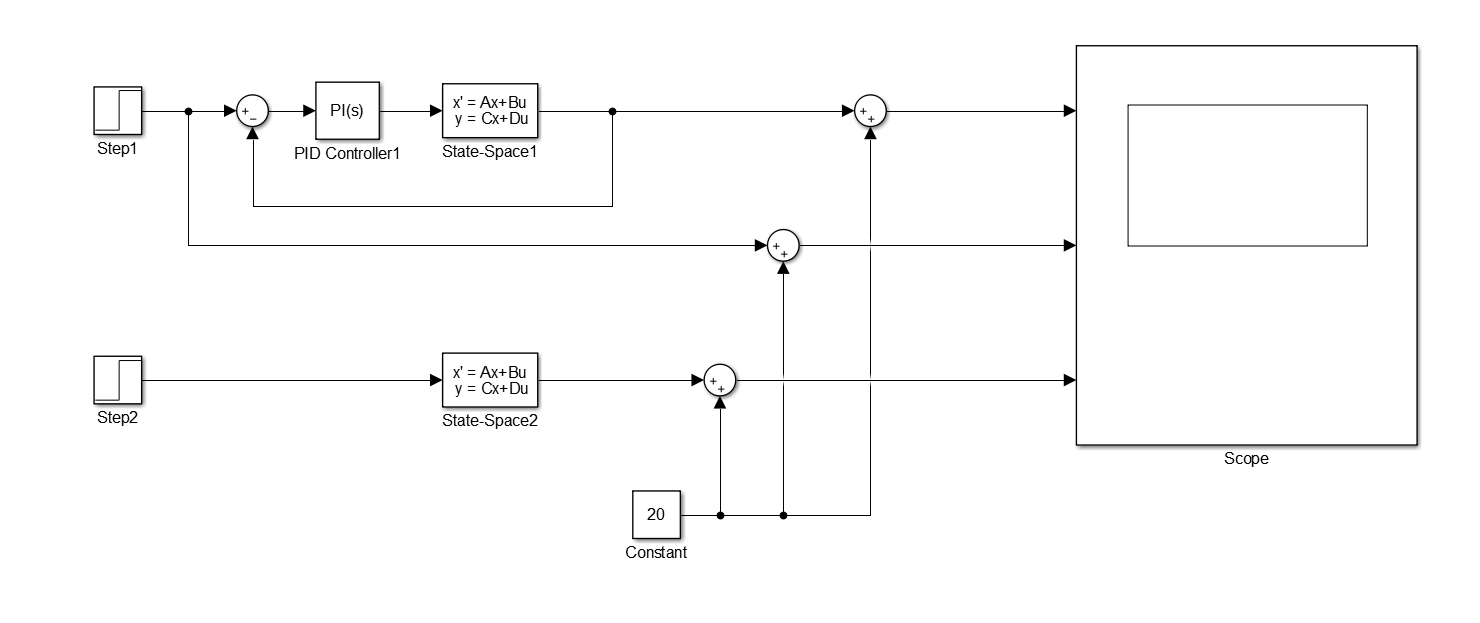
\includegraphics[width = 0.9\textwidth]{images/simulink_model}
\caption{Simulink model of the compensated and uncompensated systems}
\label{fig:1}
\end{figure}
An offset of 20$^oC$ was used to simulate room temperature.









%----------------------------------------------------------------------------------------

\chapter{Results}
Figure \ref{fig:2} shows the output of the simulation as illustrated in Figure \ref{fig:1}:
\begin{figure}[h]
\centering
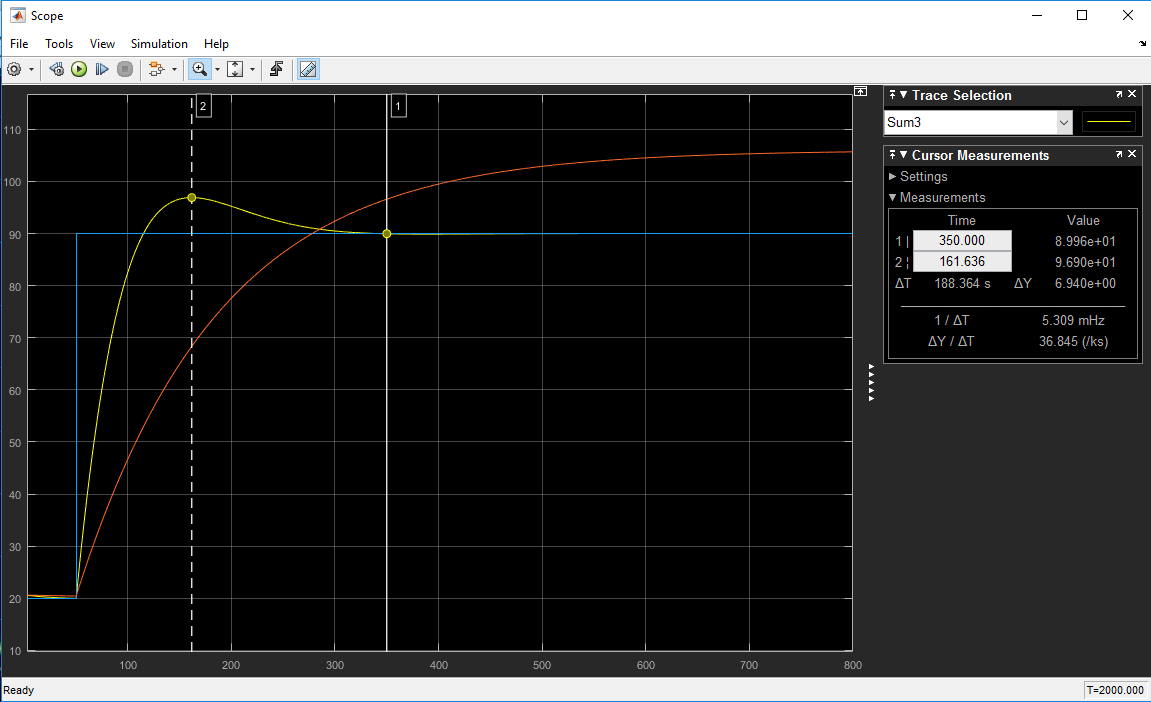
\includegraphics[width = 1\textwidth]{images/simulink_output}
\caption{Output of the simulation}
\label{fig:2}
\end{figure}

Figure \ref{fig:2} shows that the maximum value reached by the compensated system was 96.90$^oC$, and that after 300 seconds, the value was 89.90$^oC$. This relates to less than 10\% overshoot and a settling time that is significantly less than 300 seconds. The design specifications were therefore met. Table \ref{tbl:2} tabulates the results 

\begin{table}[h]
\centering
\caption{Results}
\label{tbl:2}
\begin{tabular}{llll}
\cline{1-2}
\multicolumn{1}{|l|}{\textbf{Parameter}}      & \multicolumn{1}{l|}{\textbf{Value}} &  &  \\ \cline{1-2}
\multicolumn{1}{|l|}{Settling time($T_s$)}    & \multicolumn{1}{l|}{267.7s}                   &  &  \\ \cline{1-2}
\multicolumn{1}{|l|}{Percent Overshoot(P.O.)} & \multicolumn{1}{l|}{9.85 \%}                       &  &  \\ \cline{1-2}
                                              &                                             &  & 
\end{tabular}
\end{table}
 It is also clear that the compensated system has a lower settling time than the uncompensated system. This will briefly be discussed in the conclusion.




\chapter{Conclusion}
The specifications were met and in that regard the assignment was successful. Furthermore the system from the first assignment was improved. The assignment illustrated the technical aspects of a PID implementation effectively and completely.


